\documentclass[oneside, a5paper,10pt]{article}

%------------Служебная информация, не меняй----------
\usepackage[TS1,T2A]{fontenc}
\usepackage[utf8]{inputenc}
\usepackage[english,russian]{babel}
\usepackage{indentfirst} %отступ в начале параграфа
\usepackage{amsmath,amsthm,amssymb} %математические библиотеки
\usepackage{graphicx}%Вставка картинок правильная
\usepackage{float}%"Плавающие" картинки
\usepackage{wrapfig}%Обтекание фигур (таблиц, картинок и прочего)
\usepackage{fancyhdr} %Колонтитул
\usepackage{geometry}
\geometry{
    left=1.5cm,% 1.9
    top=1.5cm,% 1.5 
    right=1.5cm,% 1.9
    bottom=1.5cm,% 1.5
    headsep=0.5cm,%
    footskip=0.5cm,%
    includehead,%
    includefoot}
\textwidth 110mm
\textheight 170mm
\linespread{1.0}
\setlength{\parskip}{3pt}
%-----------------------------------------------------

\begin{document}
%--------Колонтитул конференции - не менять------------
\pagestyle{fancy}
\fancyhead{}\fancyfoot{}
\fancyhead[C]{Мультидисциплинарная молодежная конференция Центрального университета «Научный телеграф»}
\cfoot{\thepage}
%------------------------------------------------------

%--------Название статьи, лишнюю строку удали----------
\centerline{\bf НАЗВАНИЕ ТЕЗИСОВ ПИШЕТСЯ КРУПНО} %название статьи
\centerline{\bf ВТОРАЯ И ТРЕТЬЯ СТРОЧКИ НА СЛУЧАЙ } %удали лишнее
\centerline{\bf ДЛИННОГО НАЗВАНИЯ}

\smallskip %отступ
%--------Информация об авторах -----------------------
\centerline{\bf}
\centerline{\bf \ \ И. И. Иванович$^{1,*}$,   \ \ С.~С. Сидорович $^{1,2}$}
\centerline{\bf В.~В. Владимиров$^{1}$, \ \ К.~Ф. Гаусс$^{1}$}
\smallskip
\centerline{$^{1}$ Центральный университет}
\centerline{$^{2}$ Московский физико-технический университет}
\centerline{$^{*}$\it email: ivanov@gmail.com}
%-------------------------------------------------------
\bigskip %отступ

%--------Аннотация в 3 предложения-----------------------
Это краткая аннотация твоей работы на 3--5 предложений. Выдели основные моменты своей работы. Обычно аннотация пишется в~стиле <<В работе исследовано, получено, показано, продемонстрировано>> и прочее. 
\medskip

%--------Клбючевые слова - не более 5-----------------------
\textit{Ключевые слова:} перколяция, двумерные карты, машинное обучение, математика, случайный лес. %ключевые слова разделяются запятыми

\medskip %отступ

Тезисы, или труды конференции (conference proceedings),~--- это кратко сформулированные основные положения и результаты научного исследования. Объём твоих тезисов не должен превышать \textbf{двух} страниц текста. 

Тезисы нужны для того, чтобы продемонстрировать твой новый результат, заявить о своём исследовании и ознакомиться с опытом других коллег.

В тезисах кратко изложи актуальность работы и её цель, выдели основную идею и алгоритм решения задачи. Приведи самые яркие результаты исследования и кратко их опиши. 

Ты можешь привести ссылки на литературу, которая использовалась для получения результата \cite{Ivanov24, Sidorob20, Pavlov 01}.
 
Можешь использовать формулы, таблицы, графики и тому подобное, но~это необязательно. Имей в виду, что общепризнанные вещи не приводятся в тезисах из-за их незначительного объёма.

Примеры оформления формул, таблиц и графиков --- ниже:
\begin{equation}\label{Eq1} %оформление формул
    \begin{gathered}
        F_1 = 2 \times \frac{Precision \times Recall}{Precision + Recall}; \\
        Accuracy = \frac{TP+TN}{TP+TN+FP+FN}.
    \end{gathered}
\end{equation}

Только не забывай их описывать.  

\begin{figure}[!h] %оформление рисунков
    \center
    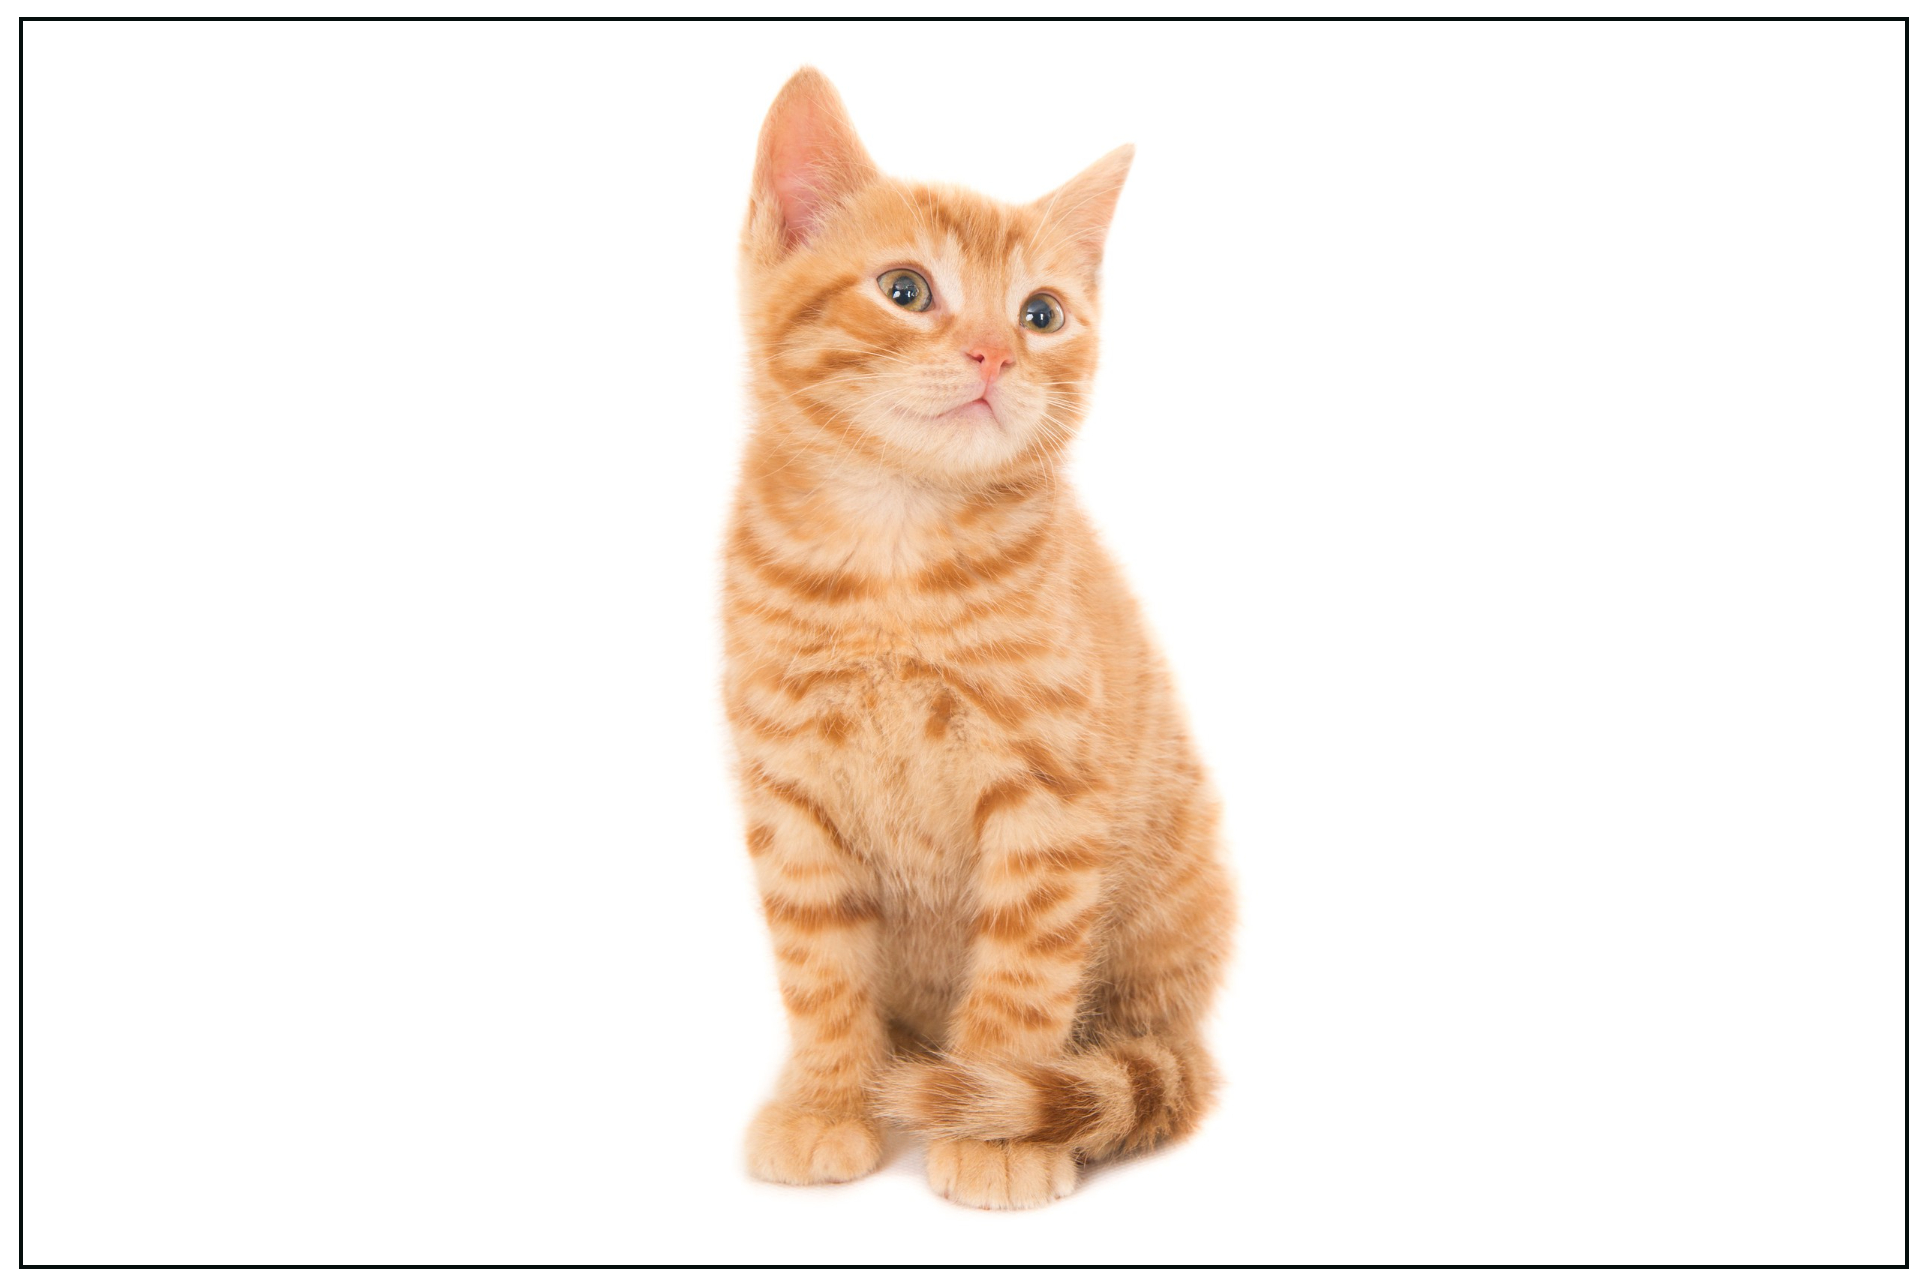
\includegraphics[width=0.45\linewidth]{cat 01.png} 
    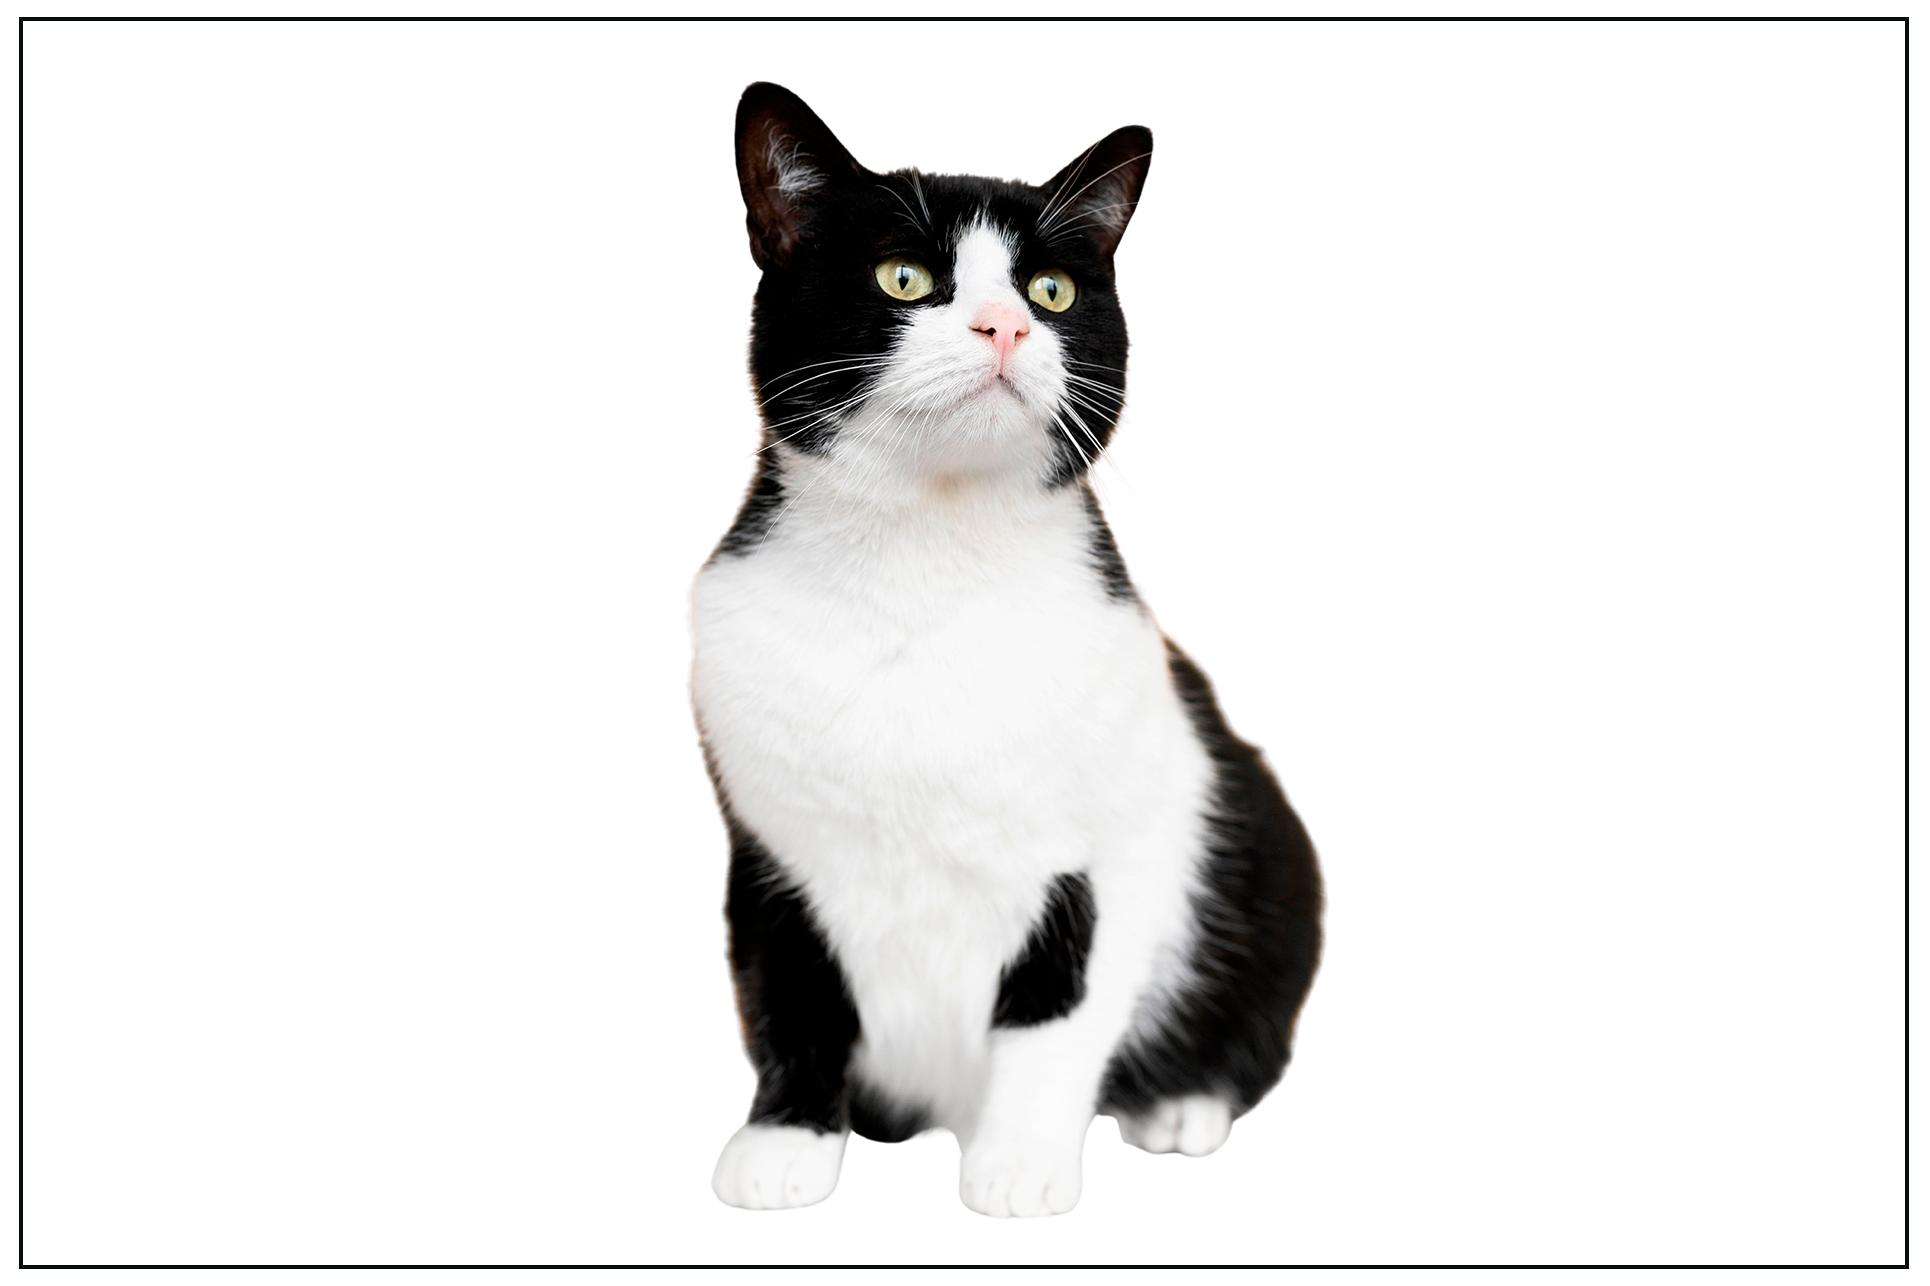
\includegraphics[width=0.45\linewidth]{cat 02.png} 
    \caption{Интенсивности излучения котиков от энергии падающего на~них потока гамма-квантов. Слева --- $E=5$ эВ, справа --- $E=10$ кэВ}
    \label{Picture1}
\end{figure}

\begin{table}[h] %оформление таблиц
\caption{\label{Tabl1} Здесь указываем подпись к таблице}
    \begin{center}
        \begin{tabular}{|c|c|}
            \hline
            \textbf{Алгоритм} & \textbf{ Ошибка}, \% \\ \hline
            Случайный лес & 5 \\ \hline 
            Линейная регрессия & 15 \\ \hline
        \end{tabular}
    \end{center}
\end{table}
Не забывай ссылаться в тексте на таблицы, графики и формулы. Используй следующее оформление: таблица \ref{Tabl1}, рисунок \ref{Picture1}, \eqref{Eq1}. 

\begin{thebibliography}{00}

\setlength{\itemsep}{1.0pt plus 1.0pt} 

\bibitem{Ivanov24}
\textit{Иванов И. И.} История человечества в эпоху расцвета магии // Вестник Хогвардса --- 2024. --- №10. --- С. 76--86.

\bibitem{Sidorob20}
\textit{Сидоров С. С., Владимиров В. В.} Введение в магическую теорию~--- М.: Интеллект, 2020. --- С. 213--412.

\bibitem{Pavlov 01}
\textit{Pavlov P. P.} How to create star from nothing at home // J. Appl. Math. –-- 2001. Vol. 3. №58. -–- P. 75--85.
\end{thebibliography}

\end{document}

